\documentclass[a4paper,12pt]{article}
\usepackage{graphicx}
\author{Didrik Jonassen, Imre Kerr}
\title{Project 1B\\ IT3708 --- Subsymbolic methods in AI}
\date{\today}

\begin{document}

\maketitle

\section{Representation and Development}
We chose to represent the chromosome as a binary vector of length $4B$. Every four bits are interpreted as a binary number, meaning that the genome codes for $B$ integers between 0 and 15. These integers are then normalized so they all sum to 1, and the resulting fractions are the troop deployment for each battle.

\section{Strategy Entropy}
Strategy entropy is a measure of how ``spread out'' the troops are for a given strategy. Putting all troops in one battle gives minimum entropy, and spreading them evenly over all battles gives maximum entropy. This is interesting because it characterizes a strategy as a single number, letting you get the gist of the strategy without having to interpret the deployment numbers themselves.

\section{EA Parameters}
\begin{tabular}{|l|l|}
\hline
Parameter & value \\
\hline \hline
Population Size & 20 \\
Mutation Rate & $\frac{1}{40B}$ \\
Crossover Rate & 100\% \\
Selection Mechanism & Fitness Proportionate \\
Selection Protocol & Generational Mixing \\
Litter size & 20 \\
Generations & 400 \\
\hline
\end{tabular}

\section{Base Case Summary}
\begin{tabular}{|c|c|c|l|}
\hline
B & R_{f} & L_{f} & Notes \\
\hline \hline
5 & 0 & 0 & Switches between various strategies putting everything on two battles \\
5 & 0 & 1 & Puts everything on battle 1 \\
5 & 0 & 0.5 & Same as (5,0,0), but weighted towards the first of the two \\
5 & 1 & 0 & Spread out, weighted towards the earlier battles \\
5 & 1 & 1 &  All on battle 1 \\
5 & 1 & 0.5 & All on battle 1 \\
5 & 0.5 & 0 & Switches between various 2-battle strategies \\
5 & 0.5 & 1 & All on battle 1 \\
5 & 0.5 & 0.5 & All on battle 1 \\
20 & 0 & 0 & Converges toward fewer battles, step by step \\
20 & 0 & 1 & Same as B = 5, but slower\\
20 & 0 & 0.5 & Same as B = 5, but slower \\
20 & 1 & 0 & Switches between different strategies involving the 10 first battles \\
20 & 1 & 1 & Same as B = 5, but slower \\
20 & 1 & 0.5 & Same as B = 5, but slower \\
20 & 0.5 & 0 & Switches between different strategies with no clear pattern \\
20 & 0.5 & 1 & Same as B = 5, but slower \\
20 & 0.5 & 0.5 & Same as B = 5, but slower \\
\hline
\end{tabular}
You'll notice that the descriptions for most the B=20 runs were the same. They did however provide us with a clearer look at what was going on, so these runs were not wasted.

\section{Signature Cases}
For each of these cases we give:
\begin{itemize}
\item{an entropy plot showing the average entropy in the population}
\item{a fitness plot showing the best, worst and average (plus/minus std.dev.) fitness in the population} 
\item{and a strategy plot, which is a visualization of the winning strategy in each generation. The horizontal axis is generations, and the vertical axis is normalized troop deployment. This plot makes it very easy to see what the dominant strategy looks like at any given point.}
\end{itemize}
\subsection{Case 1: $B=5, R_{f}=0, L_{f}=1$}
\centerline{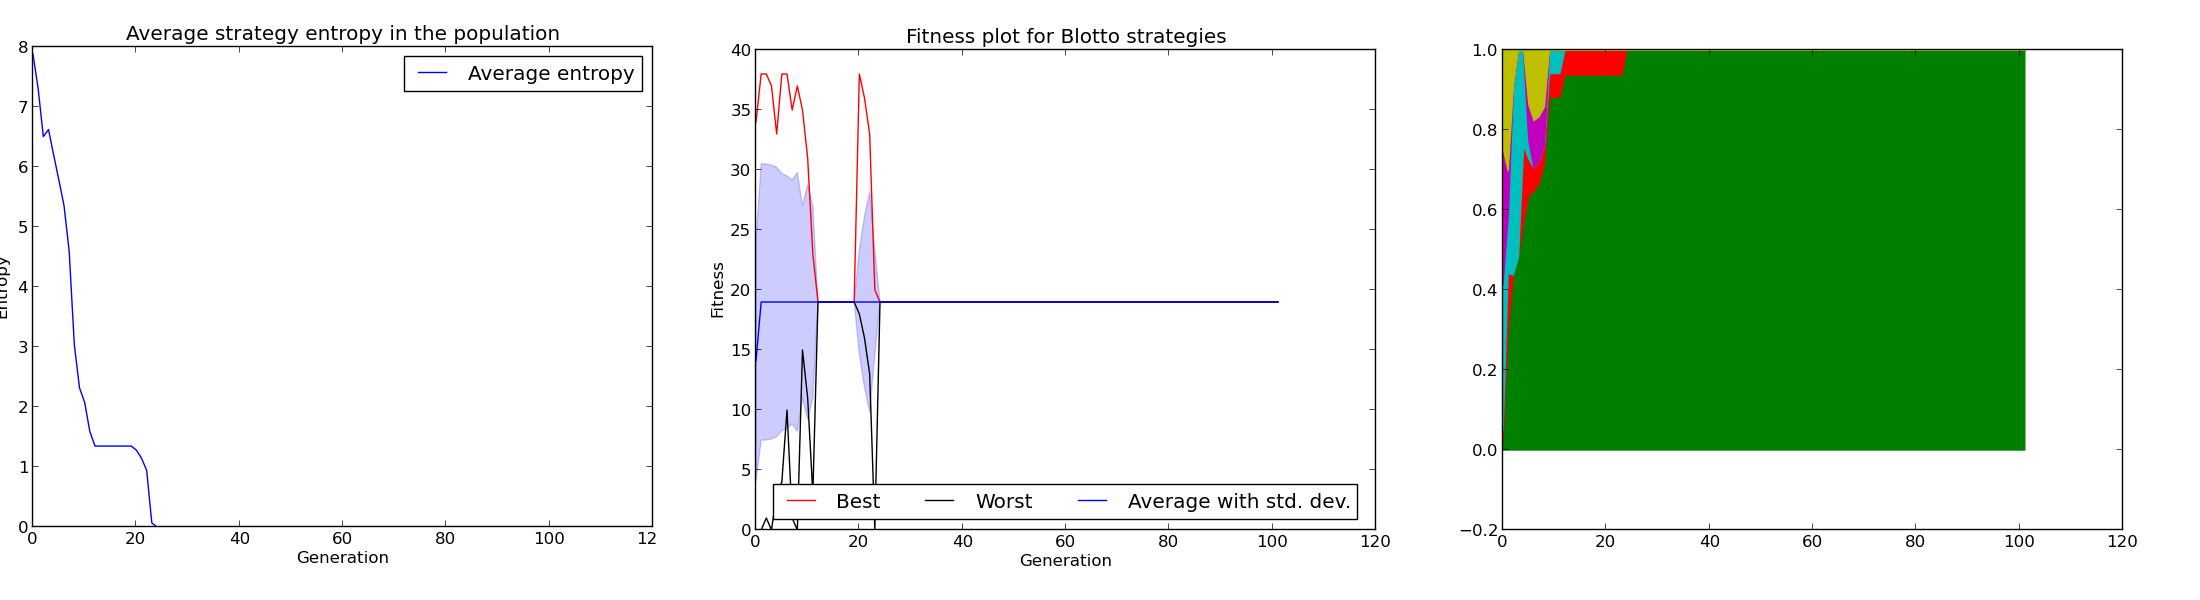
\includegraphics[width=1.2\textwidth]{case1}}
This case quickly converges towards putting all troops on the first battle. This is not surprising, since having $L_{f}=1$ means that losing the first battle will make the morale zero for all the following battles. This is true for all cases with $L_{f}=1$.

\subsection{Case 2: $B=20, R_{f}=0, L_{f}=0$}
\centerline{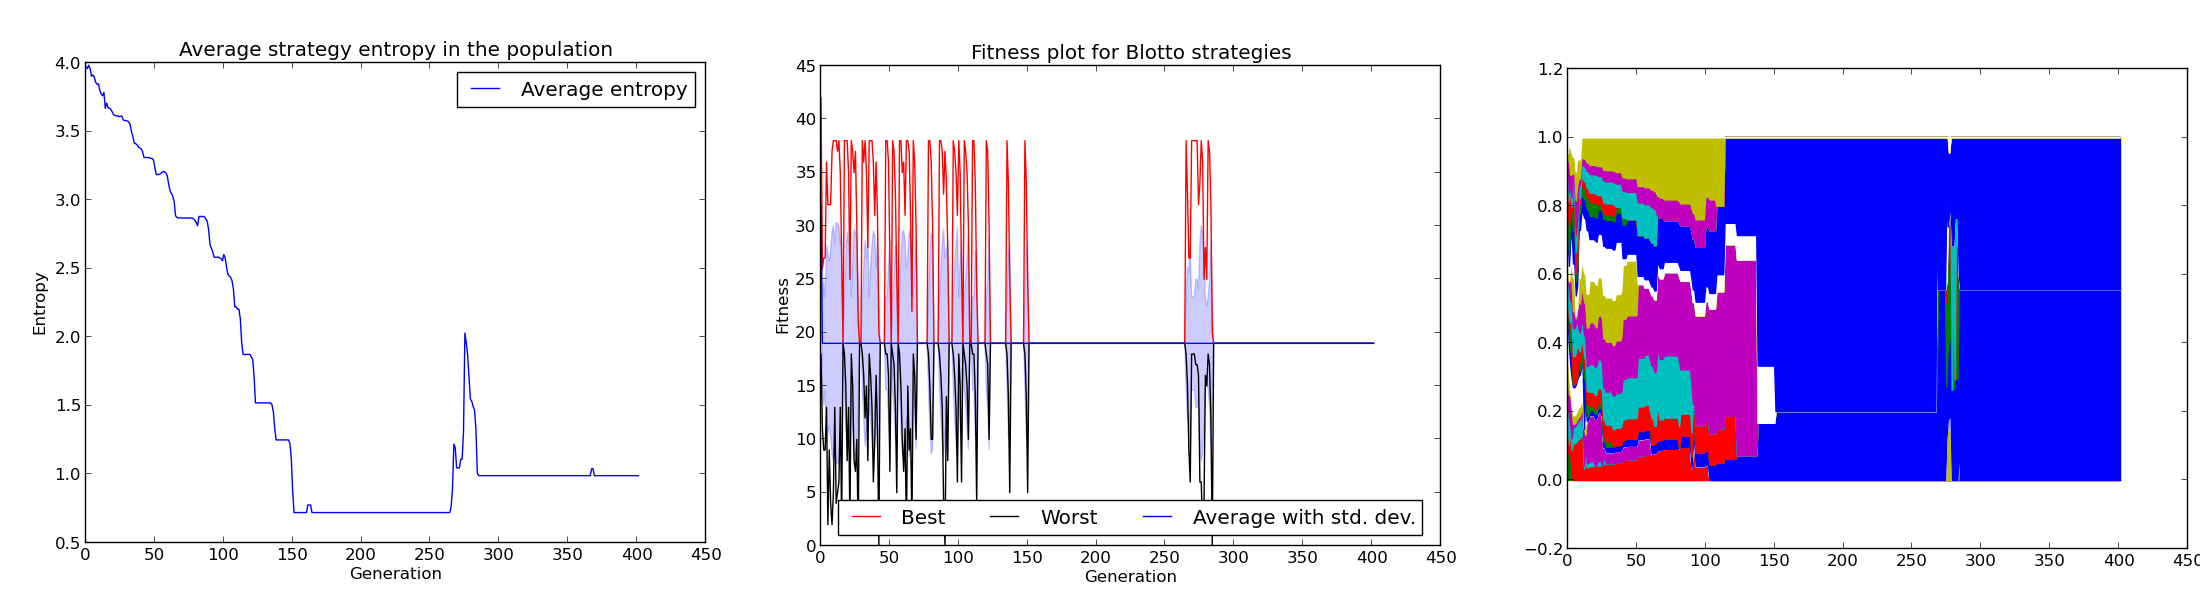
\includegraphics[width=1.2\textwidth]{case2}}
\small{(There are two distinct regions that unfortunately both happened to be blue.)}\\
This case gradually converges towards a strategy involving putting everything on two battles, with the trend being one less battle every few generations. We think this can be explained as follows: In order to mutate an n-battle strategy into an (n-1)-battle strategy that beats the original, only one of the battles needs to have a lower weight, and all the other weights will rise as a result. Conversely, if an (n+1)-battle strategy is to beat an n-battle strategy, more than one of the battles needs to get an updated value. Thus it is easier to find winning strategies with lower numbers of battles, so it converges towards lower numbers, with the limit being 2.

\subsection{Case 3: $B=20, R_{f}=1, L_{f}=0$}
\centerline{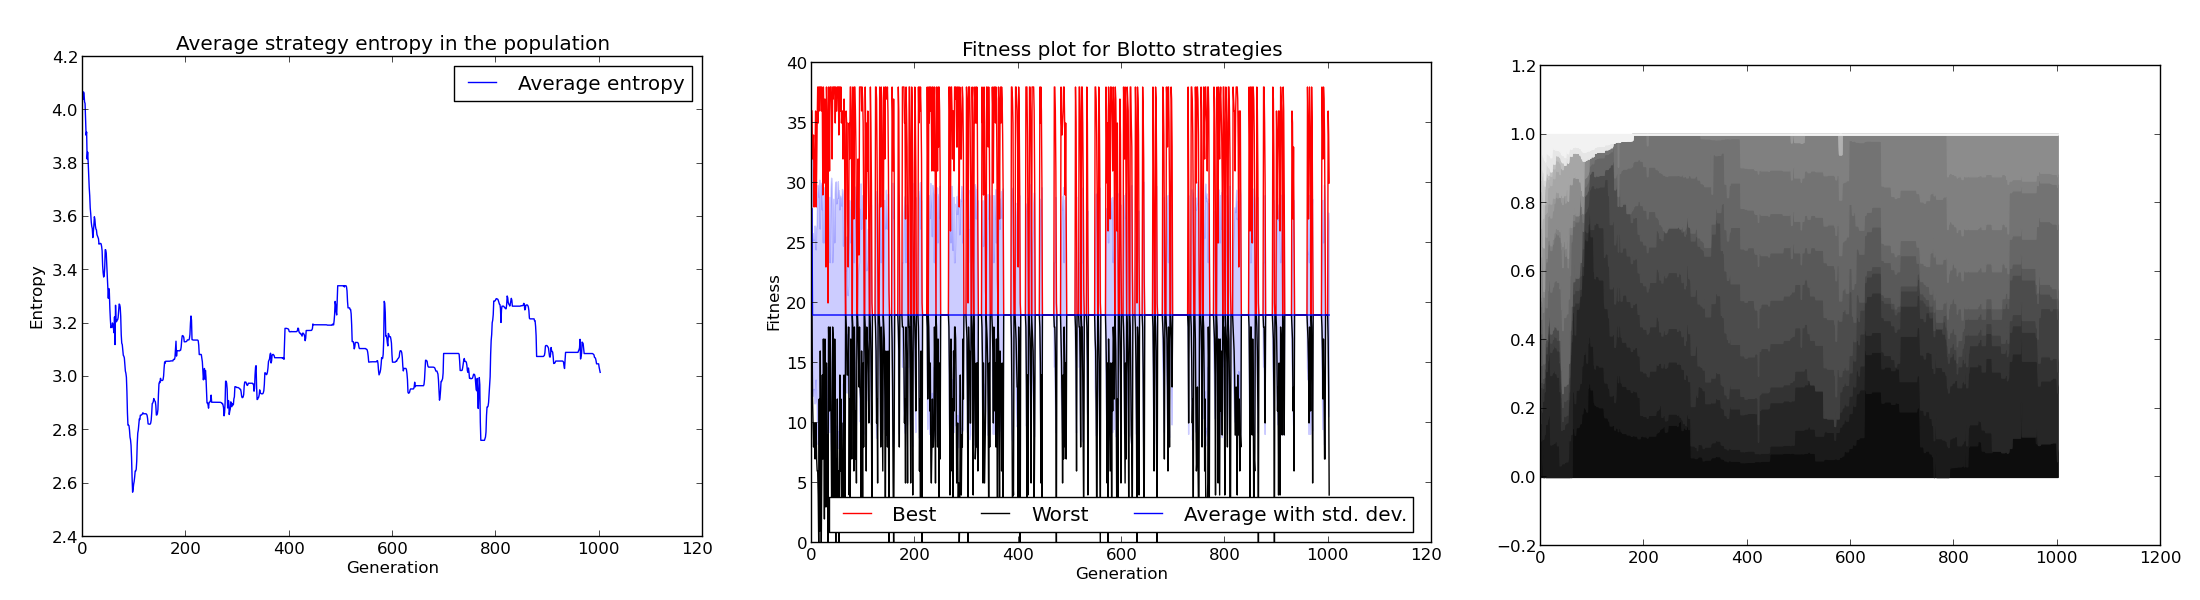
\includegraphics[width=1.2\textwidth]{case3}}
Here we see a chaotic switching between strategies involving approximately the first half of the battles. Weighting towards earlier battles makes sense due to redeployment, but other than that this one is hard to explain. We made the strategy plot greyscale for this one in order to better see which battles were included in the strategy.

\section{Brief Discussion}
In the cases where there exists an optimal solution, we see that co-evolution finds this solution quite quickly. In the more complex cases, for any given strategy there is a strategy that can beat it, and this will eventually be found. The limiting factor in these cases is how easy it is to get to that strategy by random mutation. This has parallels in biology, where most change we observe is gradual, with quantum leaps being quite rare.

\end{document}
